\section{Hardware Implementation}
\label{sec:implementation}

A possible hardware implementation of \disr{} algorithm will be
described in this section. Figure~\ref{fig:node_structure} depicts the general
structure of a node in the particular scenario of DNA nano Network-On-Chip. In particular, such a node
is composed of the following fundamental elements:

\begin{itemize}%----Start Itemize------

	\item \textbf{I/O Buffers-Transceivers:} These elements, one for
	each port, are responsible for data transmission with neighbors
	nodes. The packets received or sent are stored in specific buffers
	named input and output buffers respectively.

	\item \textbf{Switch Matrix:} Driven by a switch controller, it enables
	reciprocal connections among devices inside the node. Before segments'
	creation, this controller receives information from
	\disr{} block. After this phase, the switch controller will be driven by
	the block implementing the routing algorithm. The \emph{Switch Matrix} is
	essentially composed of a series of multiplexers and demultiplexers.

	\item  \textbf{Processing Element (PE):} It is strictly related to the
	functionality and role that the node cover inside a given network (e.g. being a
	computation or storage node).

	\item \textbf{\disr{}-Routing:} The \disr{} block contains all the hardware, control
	logic and configuration registers, needed by the implementation of the
	proposed approach. The routing algorithm receives information
	from \disr{}  which indicates the status of segments related to a
	particular node. Routing operations will take into account these
	information to obtain deadlock freedom. Both Routing
	and \disr{} are connected to the \emph{Switch Matrix} in order to receive
	packets from the input buffer. Since the packets are processed one at
	a time, a specific arbiter should be present within the \emph{Switch Matrix}
	controller. 

\end{itemize}%------End Itemize------

\begin{figure}
  \centering
  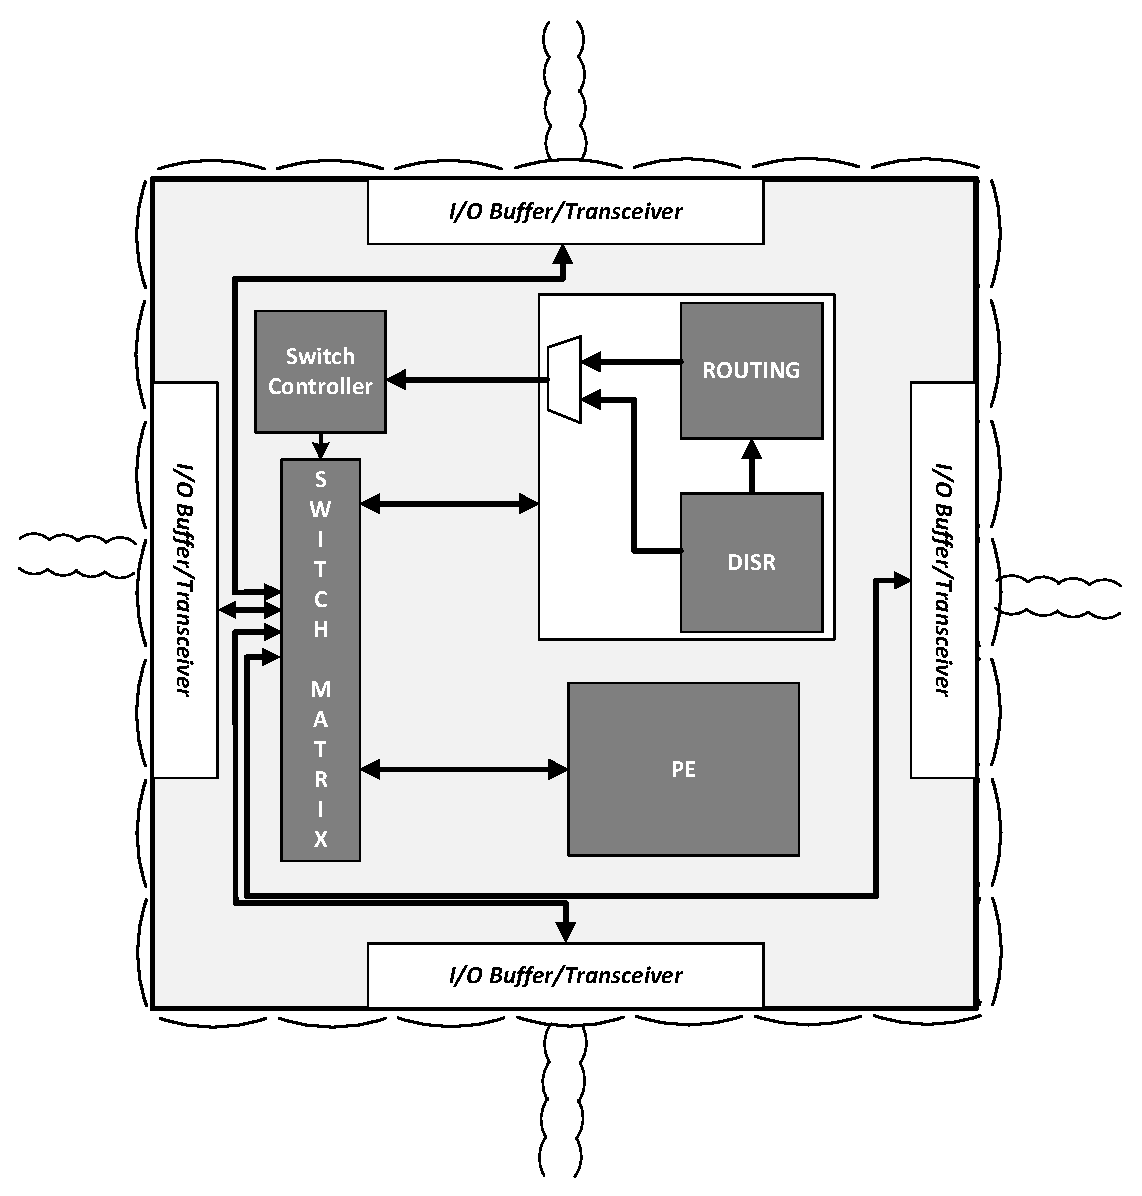
\includegraphics[width=0.45\textwidth]{pictures/node_structure.eps}
  \caption{A possible node structure tailored for a DNA nano Network-On-Chip.}
 \label{fig:node_structure}
\end{figure}
%--------------------------------------------------------------------
\subsection{\disr{} Architecture}
\label{ssec:disr_architecture}

\begin{figure}
  \centering
  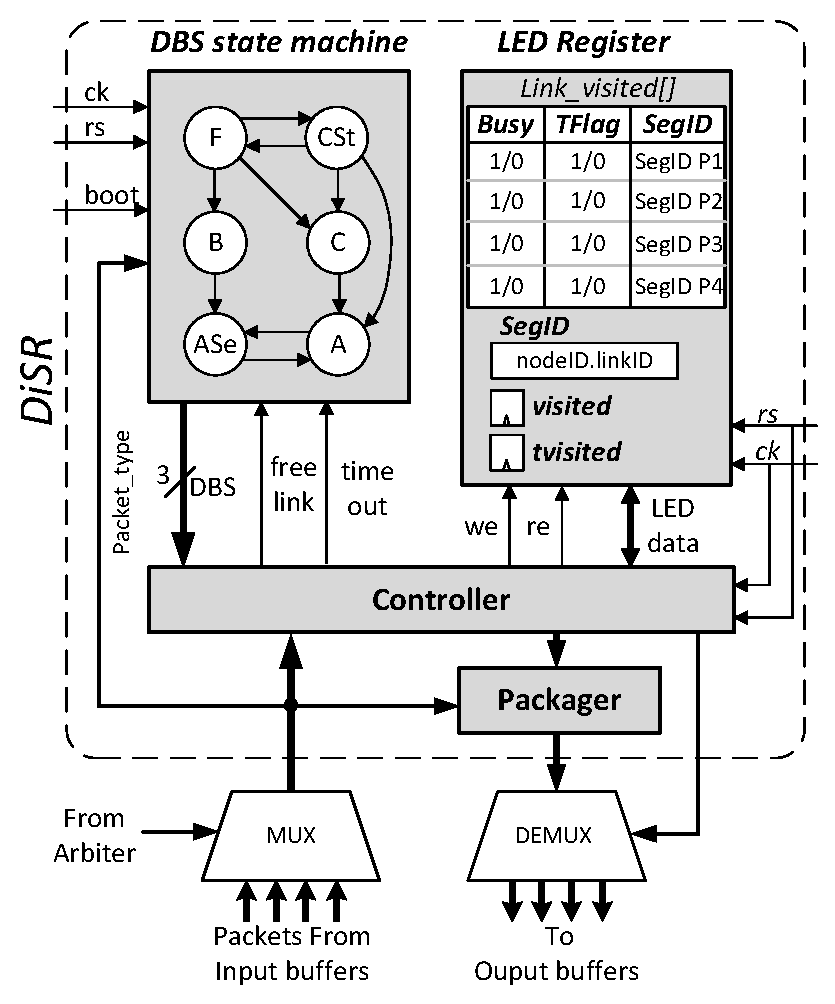
\includegraphics[width=0.40\textwidth]{pictures/disr_rtl_updated.eps}
  \caption{\emph{\disr{}} block architecture.}
 \label{fig:implementation}
\end{figure}

To give a basic estimate of the overhead needed, we focus on \disr{}-
specific components namely the control logic and configuration
registers needed to implement \disr{}. Figure~\ref{fig:implementation}
shows an architecture sketch, which mainly consists in the
following building elements:

\begin{itemize}

	\item \textbf{DBS block:}

	It takes trace of the DBS state machine, consisting of a 3-bit
	register (to cover six DBS values) and the required combinational
	logic. This block receives signals from  stored packets  in order
	to decode the packet type, and from  the control circuitry to
	change its status. The bootstrap node is selected by setting the
	boot signal to high during the initialization phase.

	\item \textbf{LED registers:}
	A set of registers stores the \emph{LED} defined in
	section~\ref{sec:disr_concepts}.  In the
	link\_visited[] table, we defined two specific registers named
	\emph{tflag} and \emph{busy}. While the first one indicates
    if the specific port of a segment is already candidate or assigned,
    the second one records if a specific port is already \emph{visited} or \emph{tvisited}.

    \item \textbf{Control circuitry:}
    This circuitry decodes incoming packet, LED
	registers and DBS, updating them when required. This block
	drives LED register according with \emph{write enable (WE)} or \emph{read enable (RE)}
	signals. Then, the resulting \emph{Ctrl-Out} drives the other
	communication resources to actuate \disr{} routing operations.

	\item \textbf{Packager:}
	Essentially it is a set of registers and multiplexers. Starting from
	an incoming packet stored in the input buffer, it updates packet's
	content before retransmission to a destination
	node.  In some cases, this circuitry builds the packet from
	scratch e.g. when a node is bootstrap and for
	the first time it should inject a \emph{STARTING\_SEGMENT\_REQUEST}. 
	Figure~\ref{fig:packager} depicts the architecture of this
	block. When a packet is created for the first time, the multiplexers 
	driven by the controller, will select information incoming from an internal 
    node such as the \emph{src\_id}. In this situation the 
	TTL field should be reset to its initial value and the \emph{segID}
	is composed of the node ID and by the output port identification 
	number.

\end{itemize}

While the elements mentioned above are part of the \disr{} circuitry,
the other devices depicted in Figure~\ref{fig:implementation} like the
multiplexer and demultiplexer are implemented outside \disr{}. In
particular, such components will be inside the \emph{Switch Matrix} (see Figure~\ref{fig:node_structure}).

\begin{figure}
  \centering
  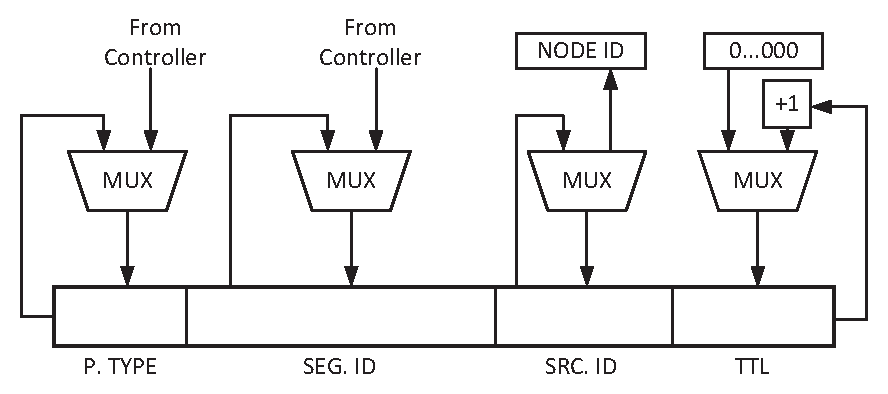
\includegraphics[width=0.40\textwidth]{pictures/packager.eps}
  \caption{Packager block.}
 \label{fig:packager}
\end{figure}

\begin{figure}
  \centering
  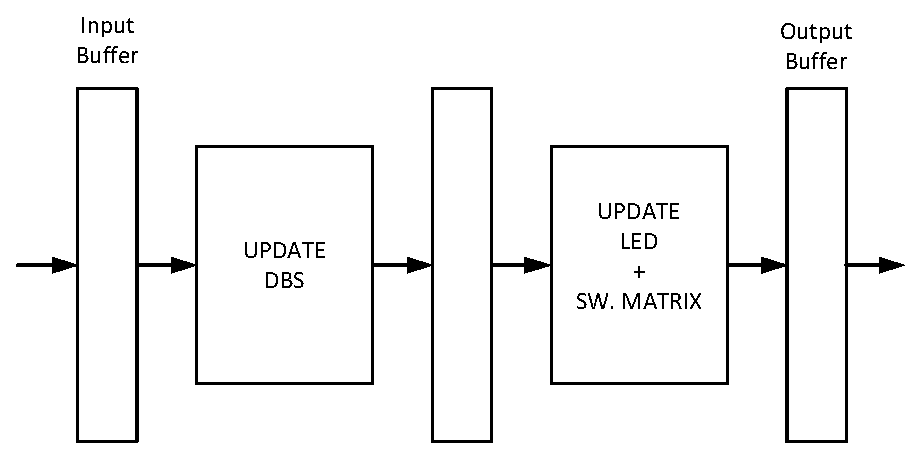
\includegraphics[width=0.40\textwidth]{pictures/pipeline.eps}
  \caption{Pipeline description of \disr{} operations.}
 \label{fig:pipeline}
\end{figure}

All the blocks described above, react with the rising edge of
the \emph{clock signal}. An asynchronous system \emph{reset} signal is
also present to restore all registers to their default values. When
this signal is set, DBS state machines for each network
node are set as \emph{Free}.  
Figure~\ref{fig:pipeline} shows the pipeline structure of the
\disr{} architecture. Packets incoming from neighbor nodes (or
generated locally) are sent to the DBS state machine in order to
ensure the status commutation. While DBS updates its state, in the
next clock cycle the control circuitry will update LED registers status and
will drive the \emph{Switch Matrix} in order to send the packets to
the right output buffer.
%--------------------------------------------------------------------
\subsection{Synthesis results: Timing, Area and Power consumption considerations}

As discussed above, one of the main design challenges of DNA Self-
Assembled systems is the limited number of resources available to implement both
computations and routing decisions for each node. Assuming a budget of
$10^4$ CNFETs for each network's node~\cite{liu_jetcs}  we estimated
the resources required to implement the entire \disr{} block. The RTL
description of the circuitry described in the last section (with an
hardware description language) has been written
and synthesized at gate-level using \emph{Synopsys Design Compiler} with 
a generic technology library (GTECH).
Considering the specific layout of each single logic element (NAND,
full-adder, latch etc.), it has been possible to get a rough estimation
of the number of transistors necessary to implement \disr{} logic.
Figure~\ref{fig:synthesys} shows the results of synthesis in terms of
number of devices (CNFETs) versus the number of network nodes while
the network scales up from $10\times10$ to $100\times100$ nodes.

\begin{figure}
  \centering
  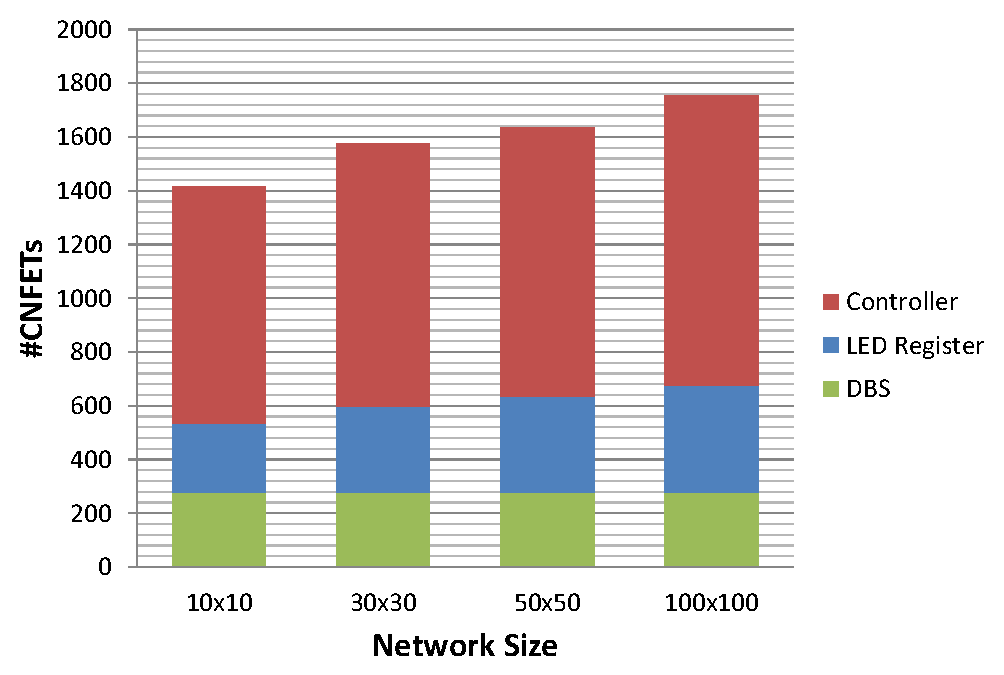
\includegraphics[width=0.50\textwidth]{pictures/synthesis.eps}
  \caption{Network size vs number of CNFETs necessary to implement
  the \disr{} circuitry.}
 \label{fig:synthesys}
\end{figure}

In particular, Figure~\ref{fig:synthesys} shows that the proposed 
implementation occupies about 17,5\% of the node budget. 
The main contribution is due to the controller circuitry followed by LED registers. 
Further, more than the
absolute number of devices itself, it is interesting to observe that
the complexity of the circuitry necessary to implement \disr{} increases
with a slowly growing trend. This is due to the
relatively simple logic of \disr{} which is almost coded with
scalable storage structures. For example, the number of registers
implementing the \emph{link\_visited[]} and \emph{link\_tvisited[]}
table follow the logarithmic function $N_{reg}=N_{port} \cdot
log_2(N)$ where \emph{Nport} is the number of the router’s ports and N is
the number of network’s nodes.

In order to have an idea of the maximum working clock frequency for
the implemented circuitry, timing results can be obtained from a 
gate-level netlist. Since a complete technology library useful for
commercial synthesis tool (e.g. Design Compiler) is not available for
this particular technology, we have
synthesized the RTL description of \disr{}, with a standard 32~nm CMOS
library, obtaining a delay of about $\mathrm{\tau_{\disr{}}=10} \ FO4$
(fan-out of four). Considering the results obtained
in~\cite{deng_isscc07}, which reports the ratio in terms of FO4
between a standard 32~nm CMOS technology and a carbon nanotube one, 
a rough delay estimation can be calculated. In particular in such work 
has been reported a ratio of:  
\begin{equation}
\mathrm{\frac{FO4_{CMOS}}{FO4_{CNFET}}=2}  
\end{equation}
Considering that F04 CMOS is about 30~ps, and the results of last
equation, a FO4 for the CNFET case is equal to about 15~ps, the working 
frequency can be computed as:
\begin{equation}
\mathrm{f_{clk}=\frac{1}{T_{max}}=\frac{1}{\tau_{\disr{}} \cdot FO4_{CNFET}}}=
\frac{1}{10\cdot 15 \cdot 10^{-12}}=6,6 GHz
\end{equation}
where $\mathrm{\tau_{\disr{}}}$ is expressed in terms of FO4.

With regard to the power consumption of the whole set of \disr{} devices: 
due to the fact that \disr{} circuitry will be active 
only once during system startup, an accurate power analisys related to switching 
activity is not provided in this work. After the setup phase, 
when all segments are mapped, the \disr{} block will stop its activity 
passing all the information related to segments to the routing
algorithm. For this reason the dynamic power falls to zero and
the only consumption is due to leakage effects. A comparison between 
the proposed circuitry and the state of the art implementation for the RPF 
algorithm, presented in~\cite{patwardhan_nanoarch06}, can show that there 
is not an appreciable discrepancy in terms of transistors cost and power 
consumption. In facts, RPF requires an overhead of about 1692 CNFET for a 
$100 \times 100$ network. Furthermore, regarding the power consumption, 
also the RPF approach has a setup phase beyond which, the consumption tends 
to zero. 
